Чтобы наглядно показать вклад микролинзирования в изменение звёздной величины \textbf{точечного источника}, используется подход, аналогичный изложенному в работе \cite{shwamb2002}. Для изображённых на Рисунке \ref{fig:histograms} карт микролинзирования были построены гистограммы, по сути, являющиеся плотностью вероятности микролинзирования и характеризующие усиление или ослабление видимой звёздной величины источника. Для всех трех проиллюстрированных случаев полная поверхностная плотность галактики-линзы остается постоянной, меняется лишь вклад звезд в полную массу системы.

\begin{figure}[H]
    \centering
	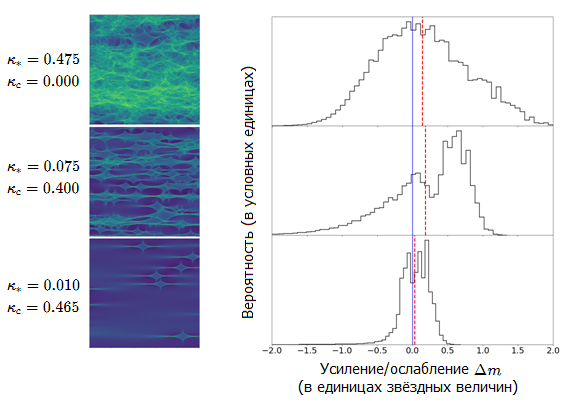
\includegraphics[scale=0.75]{pics/histograms.png}
	\caption{\textit{Слева}: карты микрокаустик, количество звёзд уменьшается сверху вниз. Размер каждой карты - $20 \times 20 R_{Ein}$. \textit{Справа}: соответствующие этим картам плотности вероятности микро-усилений (т.е. изменений звездной величины источника вследствие микролинзирования только). Сплошная голубая линия показывает $\Delta m=0$, т.е. когда звездная величина источника согласуется с теоретически ожидаемым значением макро-усиления (вследствие линзирования галактикой как целым), пунктирная красная линия - среднее по карте значение усиления. \label{fig:histograms}} 
\end{figure}

Так как микролинзирование происходит на отдельных звёздах, при уменьшении их количества (при этом величина $\kappa_*+\kappa_c$, то есть полная поверхностная плотность, сохраняется постоянной) дисперсия плотности вероятности ожидаемо уменьшается. Так же из гистограмм следует, что микролинзирование в среднем ослабляет изображение (по крайней мере, для того набора параметров, который используется для построенных карт). 
